\subsection{Density Estimation}
\label{appendix:density_estimation}

Given the strong connection between ML/AI methodologies and the theory of probability, estimating the probability distribution function  of a given dataset is of foundamental importance to understand the underlying data structure, as well as to perform various downstream tasks. In this section, we will briefly outline the basis behind the parameteric and non-parametric density estimation methods for the density estimation tasks.

\subsubsection{Parametric Density Estimation}
\label{appendix:parametric_density_estimation}

The parametric model assumes that the underlying data distribution can be modeled by the probability distribution function with a fixed parameterised functional form $p(\bm{x})\sim p_{\boldsymbol{\theta}}(\bm{x})$. This is usually the case when one has a strong physical knowledge on the prior distribution of the data, such as the normal distribution [\cref{eq:particle_velocity_distribution}] that is used to sample the initial particle velocities in the MD simulations under a given temperature $T$. Generally speaking, one can assume any well-known probability distribution functions as outlined in \cref{tab:discrete_prob_distributions} and \cref{tab:continuous_prob_distributions}. Nevertheless, the most common choice is to model the data distribution with a mixture of Gaussian distributions, which leads to the GMM [\cref{fig:multimodal_gaussian_parameter_space}]:
\begin{equation}
  \label{eq:GMM_density_estimate}
  p(\bm{x})=\sum_{k=1}^{K}\pi_k \mathcal{N}(\boldsymbol{\mu}_k,\boldsymbol{\sigma}_k).
\end{equation}
Denoting $\boldsymbol{\theta}_k=(\boldsymbol{\mu}_k,\boldsymbol{\sigma}_k)$, then the optimal parameter $\hat{\boldsymbol{\theta}}$ can be obtained through maximising the log likelihood function $\hat{\boldsymbol{\theta}}=\argmax_{\boldsymbol{\theta}}\sum_{k=1}^{K}\log p_{\boldsymbol{\theta}_k}(\bm{x})$, which, however, does not have a general solution for $K>1$ (for $K=1$, the optimum solution is given by the mean and the standard deviation of the dataset $\{\bm{x}_i\}_{i=1}^{M}$). As one can envisage, the fundamental challenge for the GMM is to determine the optimal number of Gaussian components $K$ to use, which requires some good prior knowledge on the data distribution.

\subsubsection{Non-parametric Density Estimation}
\label{appendix:non_parametric_density_estimation}

In contrary to the parametric model, the non-parametric density estimation does not assume any specific functional form for the underlying probability distribution function for the data, but trying to directly estimate the probability distribution function from the data itself. Notably, the most common choice of the non-parametric density estimation is the kernel density estimation (KDE), which, in its most general form, the probability distribution function can be expressed as
\begin{equation}
  \label{eq:KDE_density_estimate}
  p(\bm{x})=\frac{1}{nh}\sum_{i=1}^{n} k_{\boldsymbol{\theta}}\left(\frac{\bm{x}-\bm{x}_i}{h}\right),
\end{equation}
in which $k_{\boldsymbol{\theta}}$ is a kernel function [as discussed in \cref{appendix:krr}], and $h$ is the so-called bandwith parameter that controls the sharpness/smoothness of the probability distribution function. Since the kernel function typically has a high (low) value for closely (distant) spaced data points, it is intuitively to understand why this is also suitable for density estimation, as the probability distribution function will be higher in the regions where the data points are more densely distributed, and \emph{vice versa}. Again, the Gaussian kernel is probably the most common (default) choice for KDE, whereas the bandwidth $h$ critically controls the levels of the details that can be captured by the KDE-estimated probability distribution function. A common default choice for the bandwidth is the Silverman's rule of thumb,\cite{silverman1986density} which is given by $h=1.06\hat{\sigma}n^{-1/5}$, where $\hat{\sigma}$ is the standard deviation of the dataset $\{\bm{x}_i\}_{i=1}^{M}$. However, this default choice may not be optimal for all datasets, and it is often necessary to perform some parameter searches to find the optimal bandwidth that can best capture the underlying data distribution.

\subsection{Signal Decomposition Analysis} 
\label{appendix:signal_decomposition_analysis}

Signal decomposition analysis, such as the principal component analysis (PCA) and its kernelized version (KPCA), are widely used unsupervised machine learning methods for dimensionality reduction and feature extractions, which try to find a small set of `basis' that correspond to the directions of maximum variance in the data, upon which the data can be projected to obtain a low-dimensional representation.

\subsubsection{Principal Component Analysis}
\label{appendix:pca}

\begin{wrapfigure}[22]{r}{0.3\textwidth}
  \begin{center}
    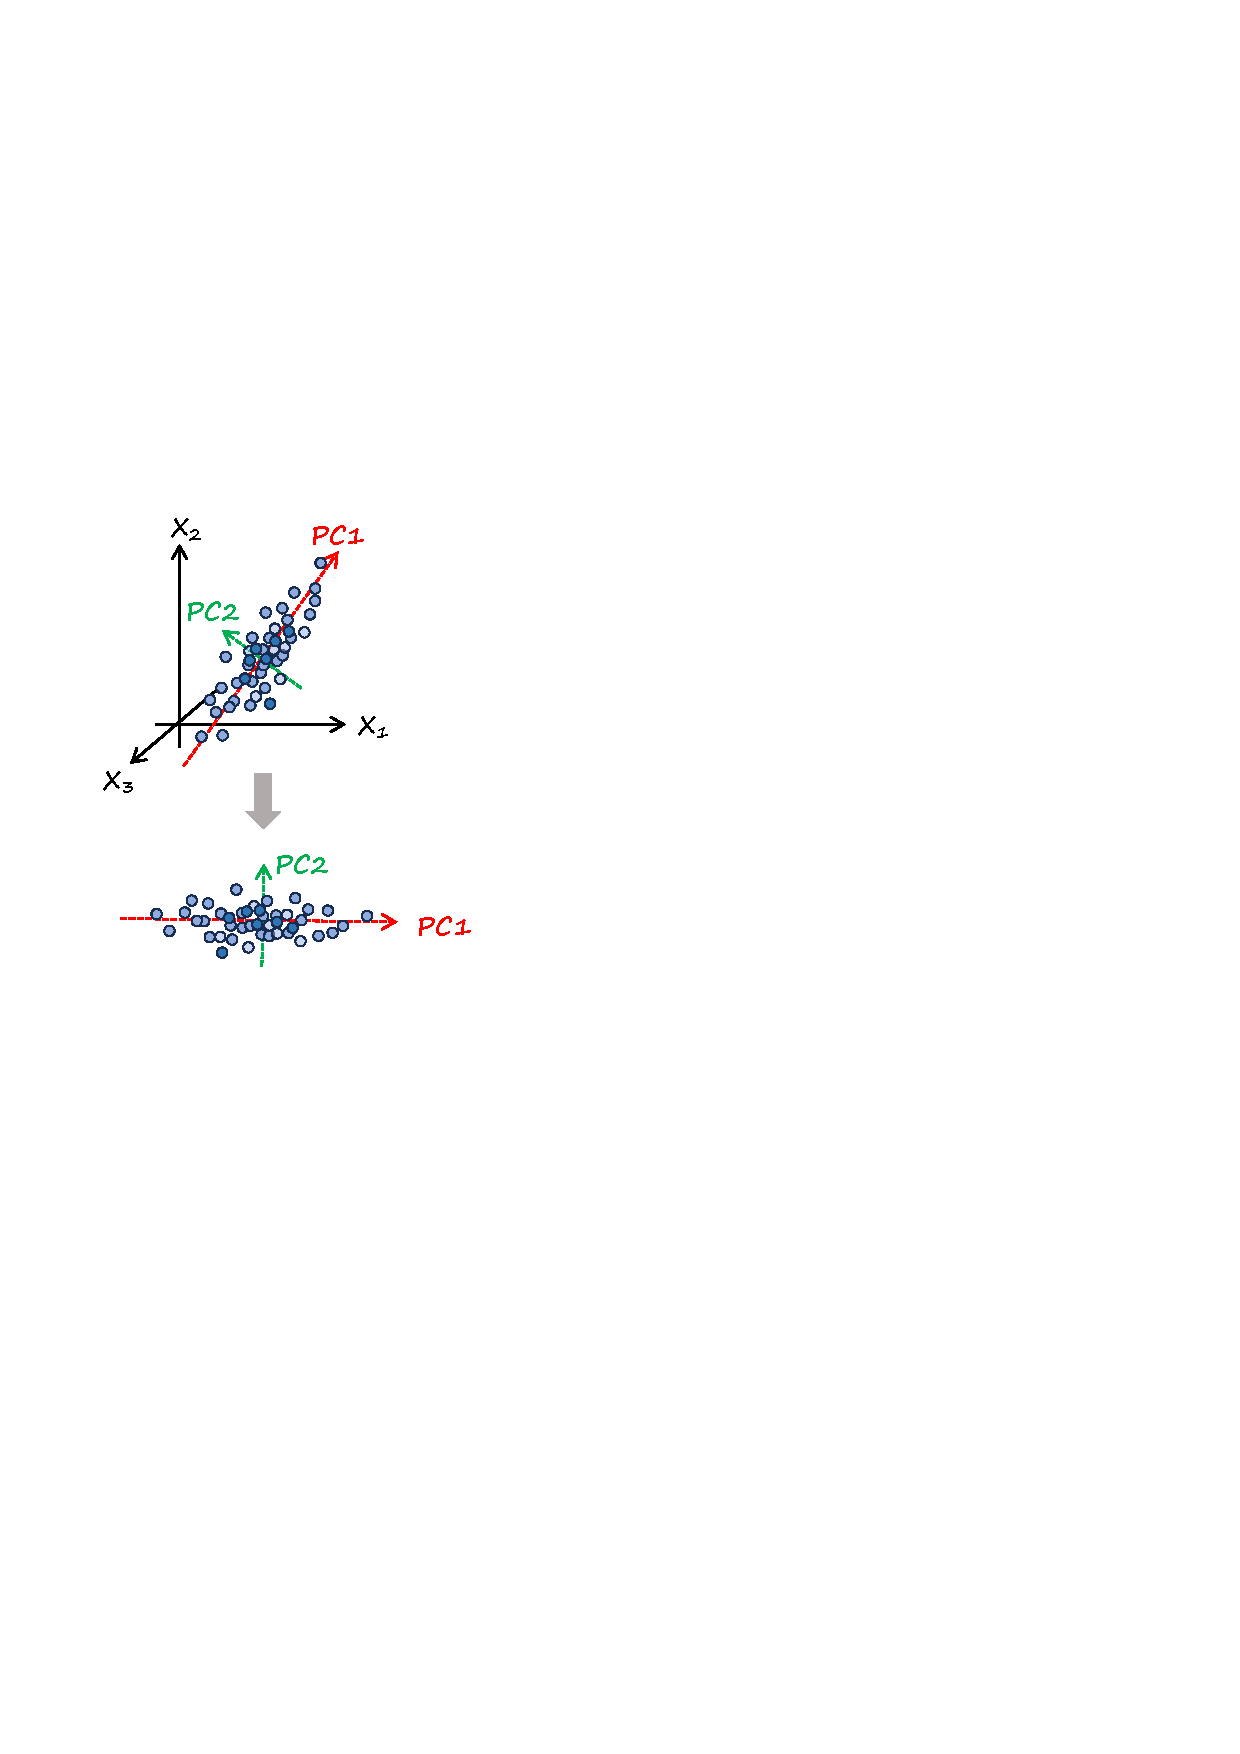
\includegraphics[width=0.3\textwidth]{PCA_illustration.pdf}
    \caption{Schematic illustration on the principal component analysis.}
    \label{fig:PCA_illustration}
  \end{center}
\end{wrapfigure}

Given a set of high-dimensional data points $\bm{X}=\{\bm{x}_i\}_{i=1}^M$ with $\bm{x}_i \in \mathbb{R}^N$ that lie in the $N$-dimensional space,  PCA\cite{jolliffe2016principal} [\cref{fig:PCA_illustration}] aims to find a set of orthogonal directions $\{\bm{v}_i\}_{i=1}^{N}$, \emph{i.e.}, the \emph{principal components}, such that along $\bm{v_1}$. the data exhibits the largest variances, followed by $\bm{v_2}$, $\bm{v_3}$, and so on.  

If we take the first $k$ $(k<N)$ dominant principal components, we can define a matrix of the principal components $\bm{V}_k=\left[\bm{v}_1,\bm{v}_2,\cdots,\bm{v}_k\right]^\top$, such that a projection of the original high-dimensional data onto the low-dimensional subspace can be obtained by the dot product of $\bm{Z}=\bm{X}\bm{W}_k$. 

To compute the principal components, we first compute the mean $\bar{\bm{x}}$ from each data point, and then compute the covariance matrix $\bm{\Sigma}=\frac{1}{M}\bm{X}^\top\bm{X}=\frac{1}{M}\sum_{i=1}^M (\bm{x}_i-\bar{\bm{x}})(\bm{x}_i-\bar{\bm{x}})^\top$. By solving the eigenvalue problem $\bm{\Sigma}\bm{v}=\lambda\bm{v}$, we can obtain the eigenvalues $\{\lambda_i\}_{i=1}^{N}$ and the corresponding eigenvectors $\{\bm{v}_i\}_{i=1}^{M}$. By sorting the eigenvectors in the descending order of their corresponding eigenvalues, the first $k$ eigenvectors with the largest eigenvalues can be selected as the principal components. Typically, the eigenvalues $\{\lambda_i\}_{i=1}^{N}$ will show a large discontinuous drop from $\lambda_k$ to $\lambda_{k+1}$,\cite{jolliffe2016principal} this can be used as a criterion to determine the optimal number of principal components $k$ to retain, which also corresponds to the intrinsic dimensionality of the data.

To show that $\bm{v}_1$ is the direction of the largest variance, we reformulate the PCA as an optimisation problem, in which we see for a unit vector $\bm{v}$ to maximise the variance of the data being projected onto it, \emph{i.e.}, $\max_{\bm{v}} \mathrm{Var}[\bm{X}\bm{v}]$, subected to the normalisation constraint of $\Vert\bm{v}\Vert_2^2=1$.  This constrained maximisation problem can be solved by the method of Lagrangian multiplier, which for this problem, read as $\mathcal{L}(\bm{v},\lambda)=\mathrm{Var}[\bm{v}^\top\bm{X}\bm{v}]-\lambda(\bm{v}^\top\bm{v}-1)$. The optimum soltion can be obtained from the equation $\nabla_{\bm{v}}\mathcal{L}(\bm{v},\lambda)=0$, which leads to the eigenvalue problem $\bm{\Sigma}\bm{v}=\lambda\bm{v}$, where $\lambda$ is the Lagrangian multiplier. The solution of this eigenvalue problem gives us the principal components $\{\bm{v}_i\}_{i=1}^{N}$ and their corresponding variances $\{\lambda_i\}_{i=1}^{N}$, which are the eigenvalues of the covariance matrix $\bm{\Sigma}$.

\subsubsection{Kernel Principal Component Analysis}
\label{appendix:kpca}

\begin{figure}[htb]
  \centering
  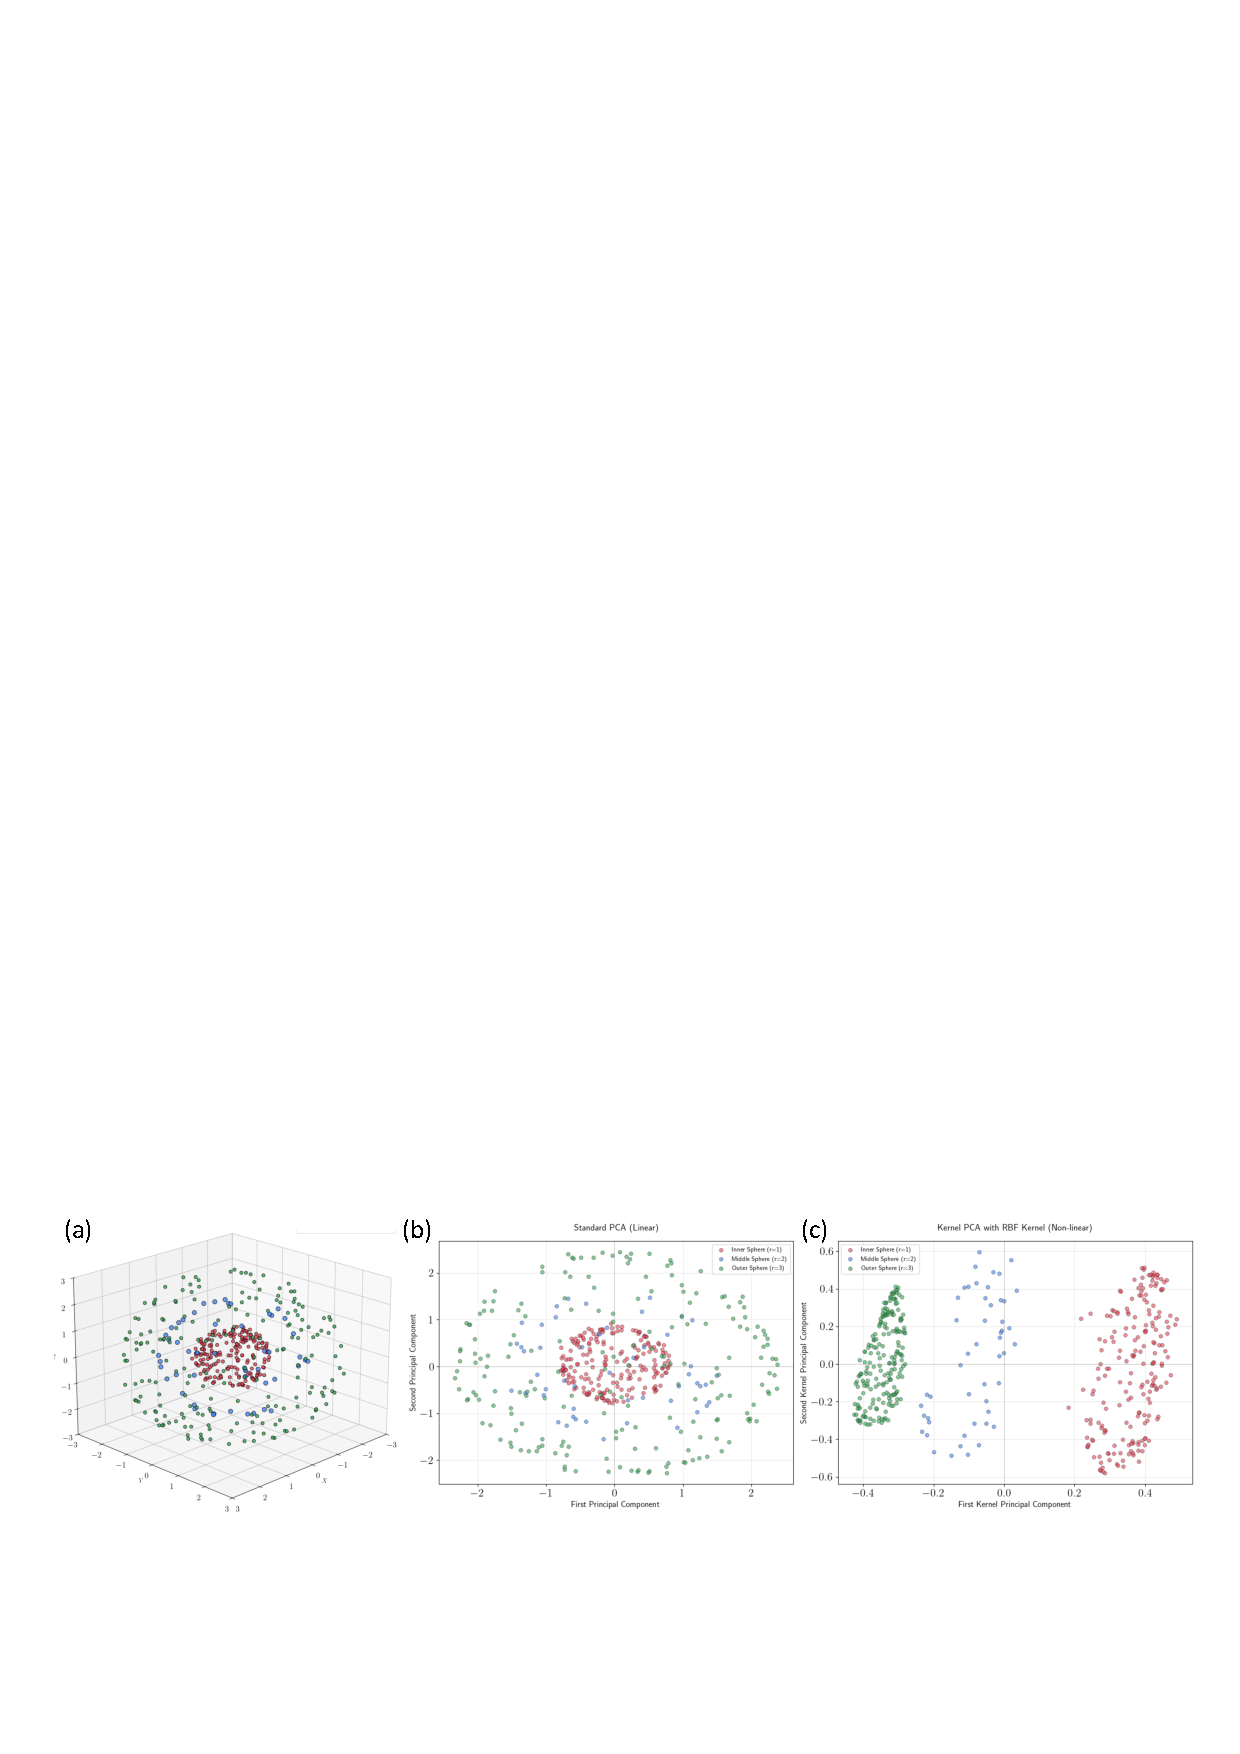
\includegraphics[width=\textwidth]{PCA_KPCA_compare.pdf}
  \caption{Dimensionality reduction analysis performed on a set of 3D concentrically distributed data points [shown in (a)], in which the results obtained from PCA (b) and KPCA (c) are compared. The KPCA analysis was performed using a radial basis function (RBF) kernel, which is defined as $k(\bm{x}_i,\bm{x}_j)=\exp(-\gamma\Vert\bm{x}_i-\bm{x}_j\Vert^2)$, where $\gamma$ is a hyperparameter that controls the width of the kernel. }
  \label{fig:PCA_KPCA_compare}
\end{figure}

Similar to the KRR [\cref{appendix:krr}] that is a kernelised version of the ridge regression [\cref{appendix:ridge_regression}] which enable the model to capture highly nonlinear relationship amongst the input data and the target variable, the KPCA\cite{scholkopf1998nonlinear}
 is a kernelised version of the PCA, in which the covariance matrix $\bm{\Sigma}$ is replaced by a kernel matrix $\bm{K}$. As dicussed above, the matrix elements of the kernel may be parameterised, that can be written as $k_{\boldsymbol{\varphi}}(\bm{x}_i,\bm{x}_j)$. When the input are feature vectors, such as structural descriptors that are built from the atomistic coordinates, themselves can also be parameterised, thus the full matrix element can be written as $k_{\boldsymbol{\varphi}}(\mathcal{F}_{\boldsymbol{\varphi}^\prime}(\bm{x}_i),\mathcal{F}_{\boldsymbol{\varphi}^\prime}(\bm{x}_j))$. Under such construction, the principal components obtained from the KPCA reflect the directions of maximum variance in the feature space, which is a high-dimensional space that is implicitly defined by the kernel, and if exits, the feature mapping function. As shown in \cref{fig:PCA_KPCA_compare}, depends on the choice of the kernel, which, in this case, a Gaussian radial basis function (RBF) kernel, the KPCA put more focus on the local structures in the data, where densly distributed data points in the high-dimensional space are more likely to be projected onto the same region within the low-dimensional space, with some tradoff in reproducing the global structure of the original data, which is more faithfully captured by the PCA.
 
\subsection{Mitidimensional Scaling}
\label{appendix:mds}

\begin{figure}[htb]
  \centering
  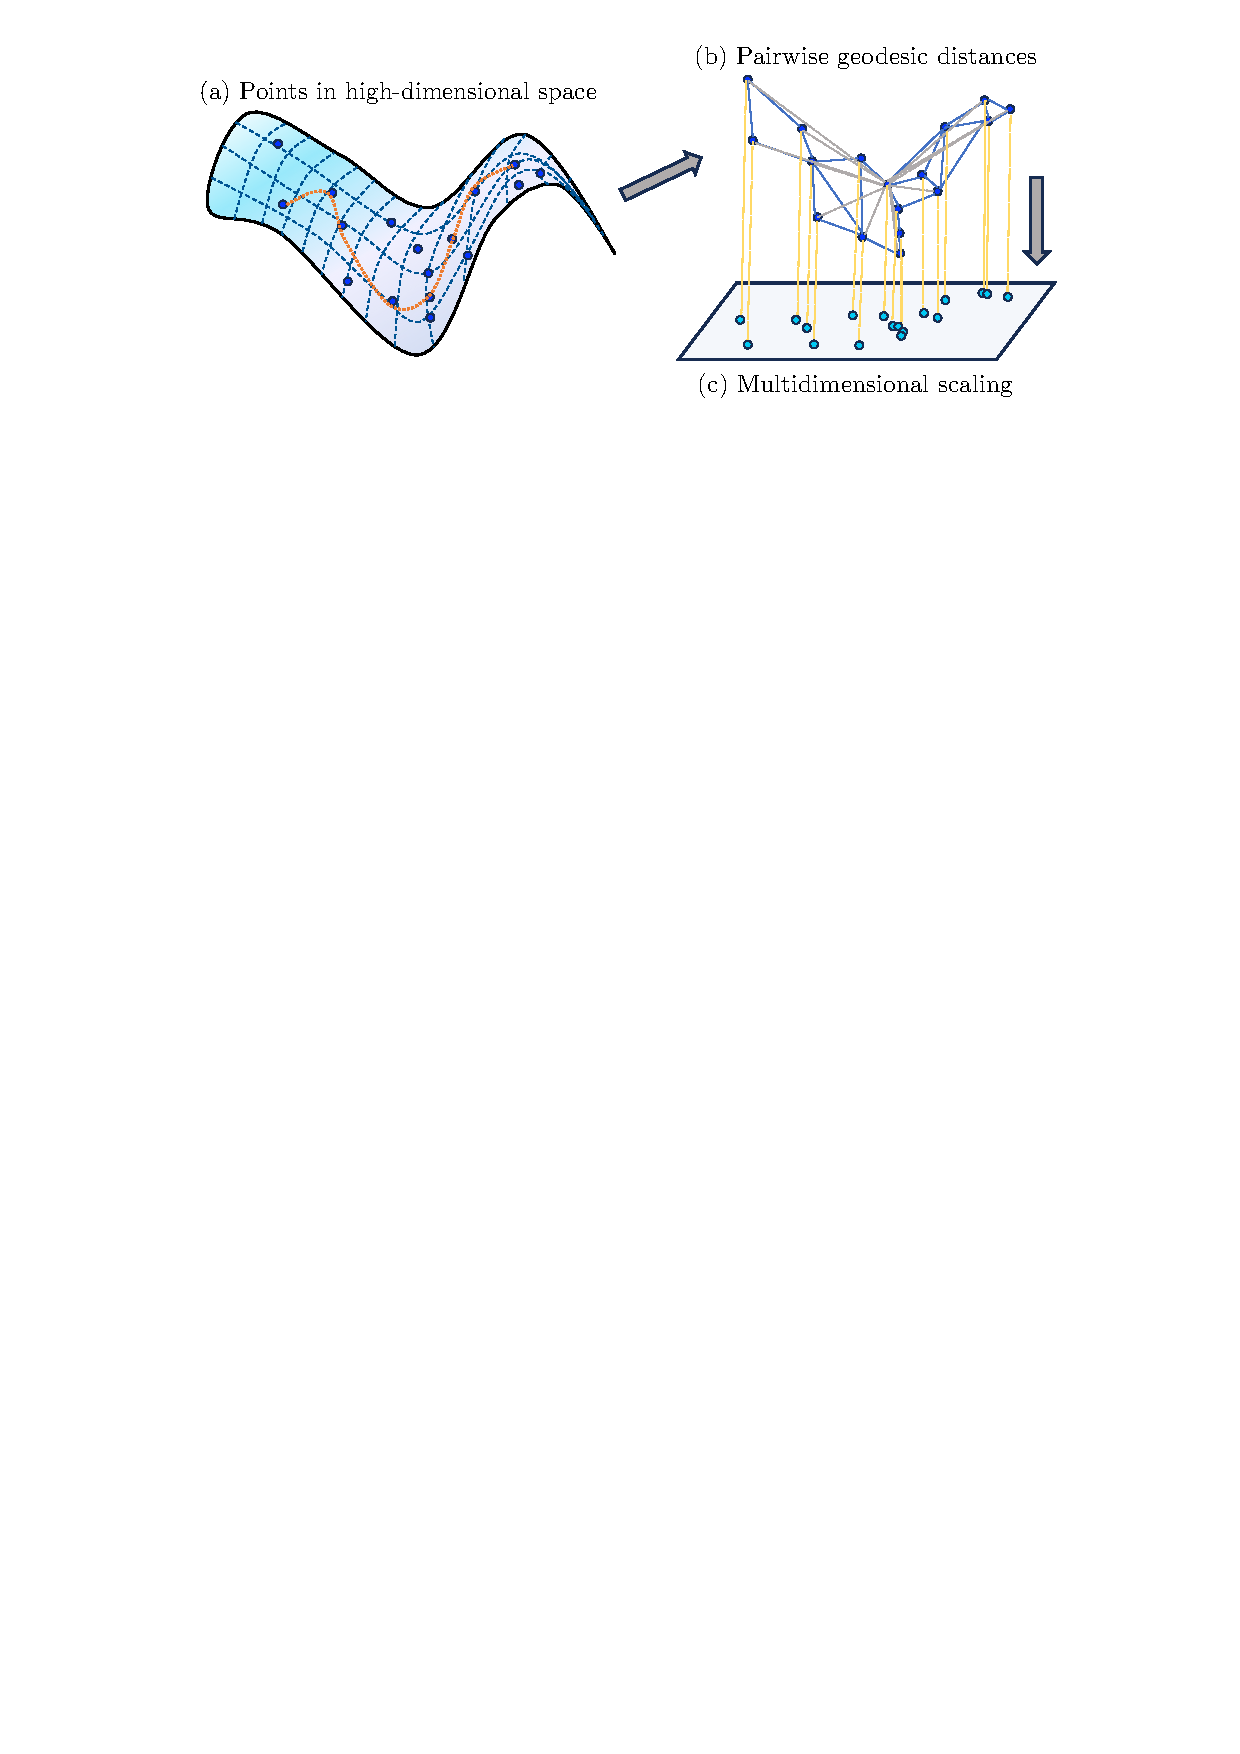
\includegraphics[width=0.8\textwidth]{mds_illustration.pdf}
  \caption{Schematic illustration on the dimensionality reduction analysis performed by the multidimensional scaling (MDS). Start from a set of data points in the high-dimensional space (a), the MDS first computes the pairwise distance matrix $\bm{D}$ (b), then the data is projected onto the low-dimensional space (c) by preserving the pairwise distances among all the points through minimising the cost function which measures the descrepency between the pairwise distances in the high- and low-dimensional spaces.}
  \label{fig:mds_illustration}
\end{figure}

Instead of focusing on extracting the highest-variant patterns among the entire dataset, sometimes, we want to put more focus on the local structure of the data, particularly the similarities and dissimilarities within each pair of data in the entire dataset. For examples, when analysing the structures sampled from an MD simulation spanned by different time intervals $\Delta t$, to understand the degrees of structural fluctuations at different time scales. For this purpose, the multidimensional scaling (MDS)\cite{borg2005modern} offers an approach to project high-dimensional data onto a low-dimensional representation by preserving the pairwise distances among all the data points [\cref{fig:mds_illustration}].

Again, starting from high-dimensional data points $\bm{X}=\{\bm{x}_i\}_{i=1}^M$ with $\bm{x}_i \in \mathbb{R}^N$, we can construct a pairwise distance matrix $\bm{R}\in\mathbb{R}^{M\times M}$, where the element $R_{ij}$ represents the distance between the data points $\bm{x}_i$ and $\bm{x}_j$. Based on the above fundamental concept behind MDS, the low-dimensional representation $\bm{Z}=\{\bm{z}_i\}_{i=1}^M$ with $\bm{z}_i \in \mathbb{R}^k$ $(k<N)$ can be obtained by minimising the cost function, which measures the descrepancy between the pairwise distances in the high- and low-dimensional spaces, \emph{i.e.}, 
\begin{equation}
  \label{eq:MDS_minimisation}
  \min_{\bm{Z}} \sum_{i<j} (R_{ij}-r_{ij})^2,
\end{equation}
 where $r_{ij}$ is the distance between the data points $\bm{z}_i$ and $\bm{z}_j$ in $\mathbb{R}^{k}$. By minimising this cost function, we can obtain a low-dimensional representation of the data that preserves the pairwise distances among all the data points as much as possible, which can be used for visualisation and further analysis. 

%However, when both $N$ and $M$ are large, the computational cost of the MDS can be very high, the computational cost associated with the na\"{i}ve MDS becomes very large and often intractable. For example, when projecting the long-time MD simulation data on macromolecules. Hence, variances of MDS algorithms have been developed to reduce the computational cost, which will be briefly introduced below.



\subsubsection{ISOMAP}
\label{appendix:isomap}

The ISOMAP\cite{tenenbaum2000global} represents one of the earliest variants of the MDS algorithm, which aims to closely map the pairwise geodesic distances among the data points in the high-dimensional manifold into the low-dimensional projection. There are three key steps behine the ISOMAP algorithm. Firstly, clusters of points in the high-dimensional space are identified based on the Euclidean distances to identify the local structures in the data. Secondly, the connecting clusters, \emph{e.g.} those that are identified by the $k$-nearest neighbour (KNN) algorithm, are furtehr connected together based on the shortest geodesic paths that are traced on the high-dimensional manifold surface. Finally, the low-dimesional representation of the data is generated by applying the classical MDS algorithms on the geodesic distances traced on the high-dimensional manifold. 

\begin{figure}[htb]
  \centering
  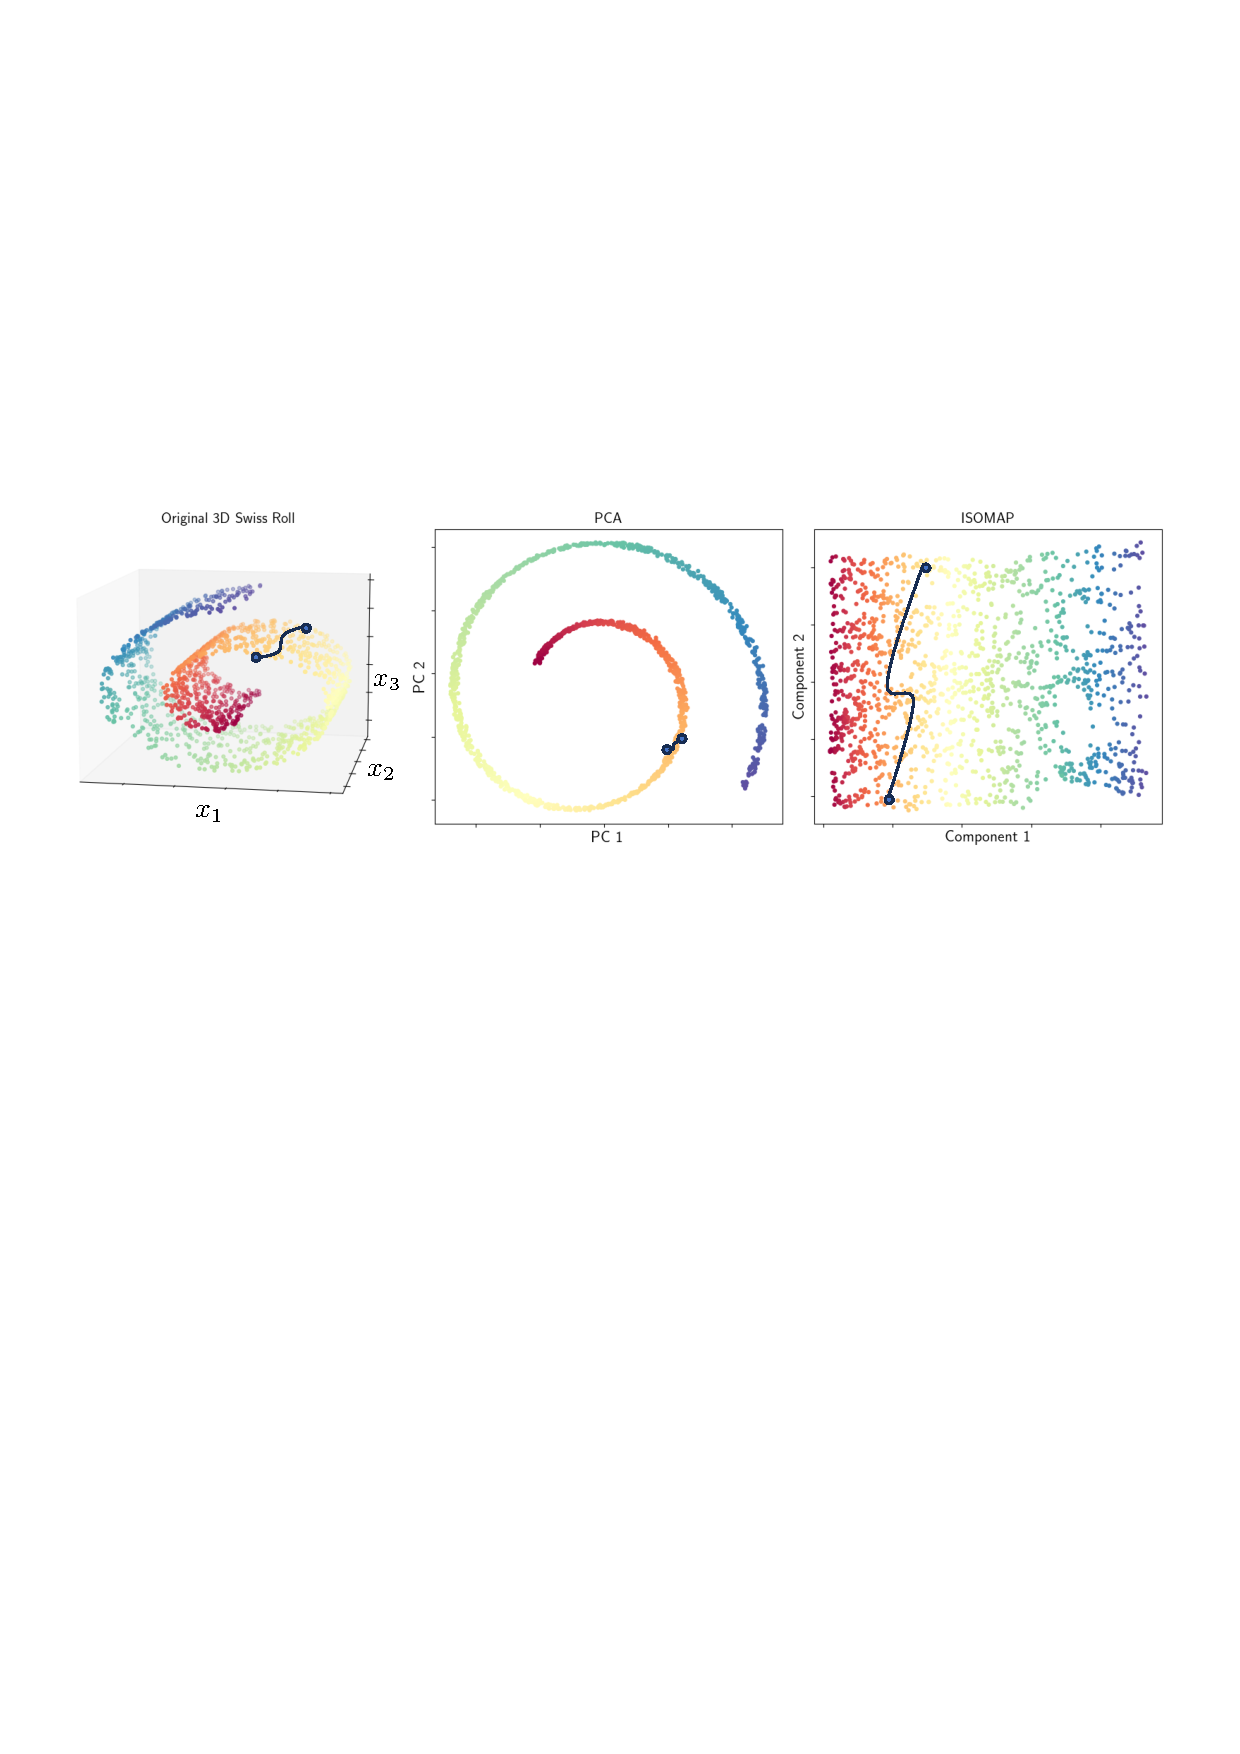
\includegraphics[width=0.9\textwidth]{PCA_ISOMAP_compare.pdf}
  \caption{Comparsion of the low-dimensional representation of the 3D Swiss roll data (left panel) obtained from the PCA (middle panel) and ISOMAP (right panel) analyses.}
  \label{fig:PCA_ISOMAP_compare}
\end{figure}

The 3D Swiss roll data is commonly used to demonstrate the differences between PCA and ISOMAP in generating the low-dimensional representation of the complex data.\cite{glielmo2021unsupervised} As also shown in \cref{fig:PCA_ISOMAP_compare}, PCA is able to capture the dominant variance of the data that occurs along the $x_1$-direction in the 3D space, but fails to reproduce the geodesic relationships along the $x_2$-directions, making the two blue points appear close to each other in the low-dimensional space. On the other hand, the ISOMAP algorithm effectively `unrolled' the original Swiss roll data, whereby the spatial relationships along the curved 3D manifold Swiss roll surface have been well preserved in the low-dimensional representation, where the two blue points are correctly projected far away from each other. 

The ISOMAP algorithm provided an attractive approach for analysing complex data, such as the free-energy landscapes for protein foldings and conformational changes in large molecules, that are simulated with MD. However, na\"{i}ve ISOMAP becomes computationally expensive, and often intractable, when both the number of data points $M$ and the dimensionality of the data $N$ are large, which is often the case for long-time (bio)molecular simuations. \cite{das2006low} proposed the landmark-based ISOMAP to overcome such a bottleneck. Here, a small set of landmark points are selected from the original data, and the geodesic distances are only computed between the landmark points and the rest of the data points. In this case, when optimising the low-dimensional representation of the data, one only needs to preserve the geodesic distances between the landmark points and the rest of the data points, which significantly reduces the computational cost of the ISOMAP algorithm. Such a landmark-based approach has also been applied in other variants of the unsupervised machine learning algorithms, such as the  KPCA\cite{zeng2023mechanistic} and sketch-map\cite{ceriotti2011simplifying} discussed below, to reduced the overall computational cost for analysing large datasets. Even with such a landmark-based approach, the ISOMAP algorithm can still be computationally expensive when applied to analyse large datasets. In the original study published in 2006,\cite{das2006low} analysis perofmed on the folding trajectory of a small protein cost $\sim$500 CPU hours.
 
\subsubsection{Diffusion Map}
\label{appendix:diffusion_map}

The diffusion map algorithm was first proposed by \citet{coifman2006diffusion} and was reviewed in the work by \citet{ferguson2011nonlinear} as an unsupervised ML method for analysing the molecular simulation data. The inspiration behind the diffusion map is by realising the fact that the dynamics of a complex system, such as the conformational changes in macromolecules, are governed by a small number of slow modes, whereas the remaining fast degrees of freedom couple to them effectively as stochastic noise. Furthermore, the evolution of the system is a Markovian process, which depends only on the instaneous state, not its previous history. Hence, it is critical that we can extract these fundamental underlying slow modes, to facilitate the understanding of the system dynamics,  parameterising the meaningful dynamic models to characterise the free energy surfaces, as well as provide robust classification of the metastable and stable configurations. 

Starting from a set of high-dimensional samples $\bm{X}=\{\bm{x}_i\}_{i=1}^M$ with $\bm{x}_i \in \mathbb{R}^N$, we first construct a Gaussian kernel matrix $\bm{K}$, where the matrix element is computed with a parameterised Gaussian function $k_\sigma(i,j)=\exp(-\Vert \bm{x}_i-\bm{x}_j\Vert_2^2/2\sigma^2)$. This can be considered as a soft-thresholding operation to retain information in which the pairwise distance between a given pair of data is of the similar order of $\sigma$, which allows us to synthesise distinct embeddings of disconnected sub-regions of the global energy landscape. This can be achived by first computing the corresponding normalised right-stochastic Markov transition matrix $\bm{P}$ can be obtained by normalising the kernel matrix $\bm{K}$ as $\bm{P}_{ij}=\bm{K}_{ij}/\sum_{i=1}^M K_{ij}$, and its corresponding eigenvalues $\{\lambda_i\}_{i=1}^M$ and eigenvectors $\{\bm{\psi}_i\}_{i=1}^M$ in the descending order of the eigenvalues. From here, the diffusion map embedding is defined as the mapping of the $i$-th snapshot onto the $i$-th component of each of the top $k$ non-trivial eigenvectors of the $\bm{P}$ matrix as $\bm{z}_i=[\psi_1(i),\psi_2(i),\cdots,\psi_k(i)]^\top$. Essentially, the diffusion distance, which is related to the Markov transition matrix, provides an indication on how easy the system can diffuse between two configurations $\bm{x}_i$ and $\bm{x}_j$, which is then reflected from the diffusion map embedding.


\subsubsection{\textit{t}-Distributed Stochastic Neighbour Embedding}
\label{appendix:t_sne}

The basic idea behind the $t$-distributed stochastic neighbour embedding ($t$-SNE)\cite{van2008visualizing} shares some similarity with KPCA using a Gaussian RBF kernel, in which the dimensionality reduction focuses on preserving the local spatial relationship among data that lie closely to each other in the high-dimensional space, whereas the relationship among the distant data points is down weighted/rejected. It is formulated based on a probabilistic model that describes the similarity between data points in the high-dimensional space and the low-dimensional space, in which we can define a probability for any point $\bm{x}_j$ to be a neighbouring point to $\bm{x}_i$ in the high-dimensional space as
\begin{equation}
  \label{eq:prob_high_d_distance}
  p(j|i)=\frac{\exp(-\Vert\bm{x}_i-\bm{x}_j\Vert_2^2/2\sigma_i^2)}{\sum_{k\neq j}\exp(-\Vert\bm{x}_i-\bm{x}_k\Vert_2^2/2\sigma_i^2)},
\end{equation}
in which $\sigma_i$ is a hyperparameter that controls the how closes two points may be considered as neighbours. Similarly, we can define a probability for any point $\bm{z}_j$ to be a neighbouring point to $\bm{z}_i$ in the low-dimensional space as:
\begin{equation}
  \label{eq:prob_low_d_distance}
  q(j|i)=\frac{(1+\Vert\bm{z}_i-\bm{z}_j\Vert_2^2)^{-1}}{\sum_{k\neq j}(1+\Vert\bm{z}_i-\bm{z}_k\Vert_2^2)^{-1}},
\end{equation}
where the Student's $t$-distribution with one degree of freedom is used to compute the similarity between data points in the low-dimensional space, which has heavier tails than the Gaussian distribution, thus can better capture the local structure of the data. The low-dimensional representation $\bm{Z}=\{\bm{z}_i\}_{i=1}^M$ can be obtained by minimising the Kullback-Leibler divergence between the two probability distributions $\mathcal{D}_{\mathrm{KL}}(p\Vert q)$, which is typically solved by gradient optimisations.


\subsubsection{Sketch-Map}
\label{appendix:sketch_map}

Generally, the distance metric used to construct the pairwise distance $R_{ij}$ (in high-dimensional space, or $r_{ij}$ in the low-dimensional space) are all normalised such that $R_{ij}\in[0,1]$. As such, ISOMAP is a procedure that focuses on preseving the information $\forall R_{ij}\in[0,1]$, whereas diffusion map and $t$-SNE are more focused on preserving the local structure of the data $\forall R_{ij}\in[0,\sigma]$.  The general idea behind the sketch-map\cite{ceriotti2011simplifying} is to provide a more flexible approach to preserve the pairwise distance information on length-scales that are particularly interesting in the high-dimensional space, which recasts the cost function in \cref{eq:MDS_minimisation} as
\begin{equation}
  \label{eq:sketch_map_cost_function}
  \min_{\bm{Z}} \sum_{i<j} \left[s_{R}(R_{ij})-s_{r}(r_{ij})\right]^2,
\end{equation}    
with a non-linear sigmoid function parameterised by $\sigma$, $a$, and $b$ defined as
\begin{equation}
  \label{eq:sketch_map_sigmoid_function}
  s(x)=1-\left(1+(2^{a/b}-1)(x/\sigma)^a\right)^{-b/a}.
\end{equation}

\subsection{Clustering Analysis}
\label{appendix:clustering_analysis}

In this section, we will briefly introduce the K-mean clustering algorithm,\cite{mcqueen1967some} which will provide some fundamental understanding on the process of clustering analysis. This will be followed by a brief introduction on the density-based spatial clustering of applications with noise (DBSCAN)\cite{ester1996density} and its hierarchical variant,\cite{campello2015hierarchical} which are most widely used in molecular and materials modellings.

\subsubsection{K-Means Clustering}
\label{appendix:k_means_clustering}

\begin{figure}[htb]
  \centering
  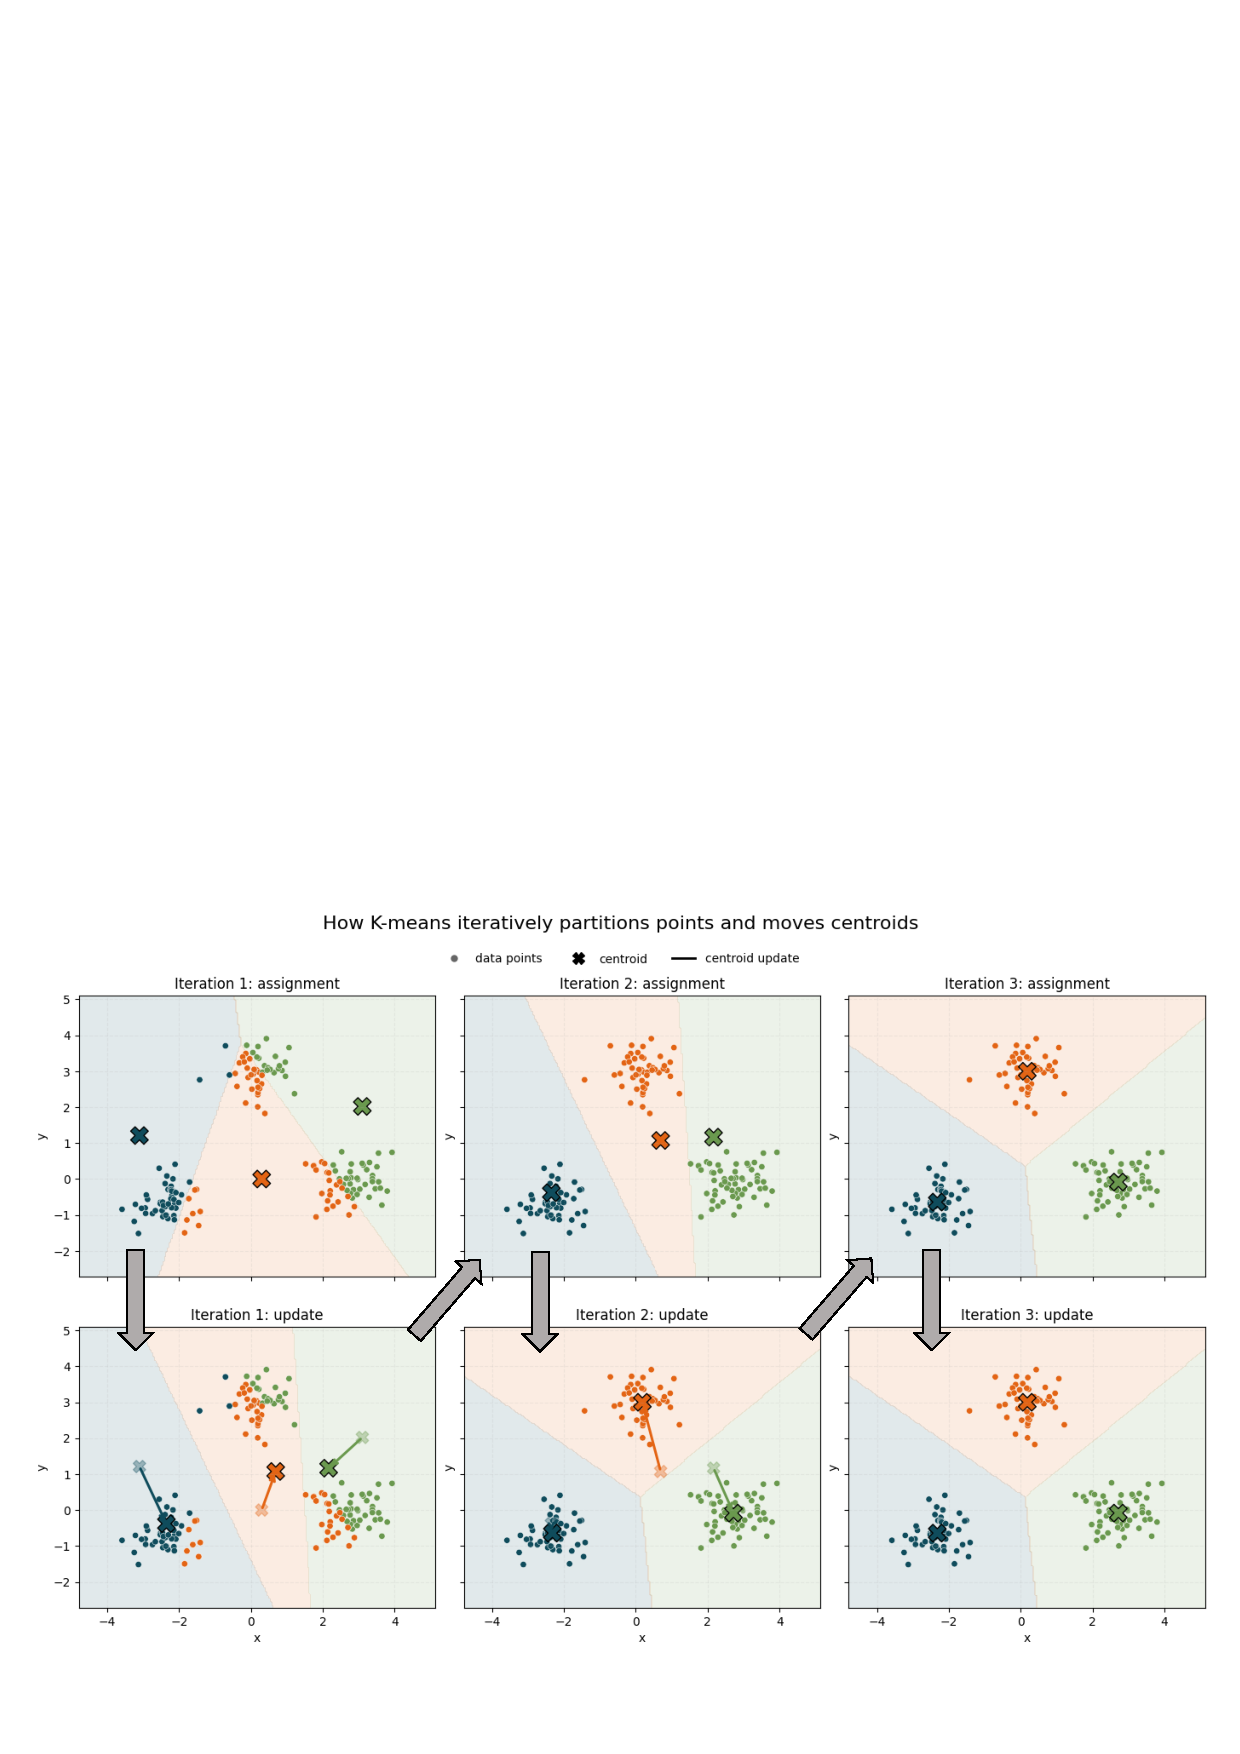
\includegraphics[width=0.8\textwidth]{K_mean_clustering.pdf}
  \caption{Schematic illustration on the process of K-means clustering analysis.}
  \label{fig:K_means_clustering}
\end{figure}

The basic process behind the K-means clustering algorithm is schematically illustrated in \cref{fig:K_means_clustering} for a set of 2D data points $\{\bm{x}_i\}_{i=1}^{M}$ ($\bm{x}_{i}\in\mathbb{R}^2$). The key hyperparameter for the algorithm is the number of clusters $K$, which is typically assigned based on some prior knowledge on the data. The algorithm starts with the random assignment of the positions for $K$ cluster centroids $\{\bm{c}_k\}_{k=1}^K$ ($\bm{c}_{k}\in\mathbb{R}^2$),  each data point is then assigned to the cluster with the closest centroid, which can be mathematically expressed as $\mathrm{argmin}_k \Vert\bm{x}_i-\bm{c}_k\Vert_2^2$. After this, the mean position of the data points within each cluster is computed as $\bar{\bm{c}}_k=\frac{1}{N_k}\sum_{i=1}^{N_k} \bm{x}_i$ for all $N_k$ data points that belong to the $k$-th cluster. This allows the cluster centroids to be updated to $\bar{\bm{c}}_k$, at which the algorithm cycle repeats again from the assignment of data points to clusters, until all the cluster centroids converge to the converged positions.

\subsubsection{DBSCAN Clustering}
\label{appendix:DBSCAN_clustering}

\begin{figure}[htb]
  \centering
  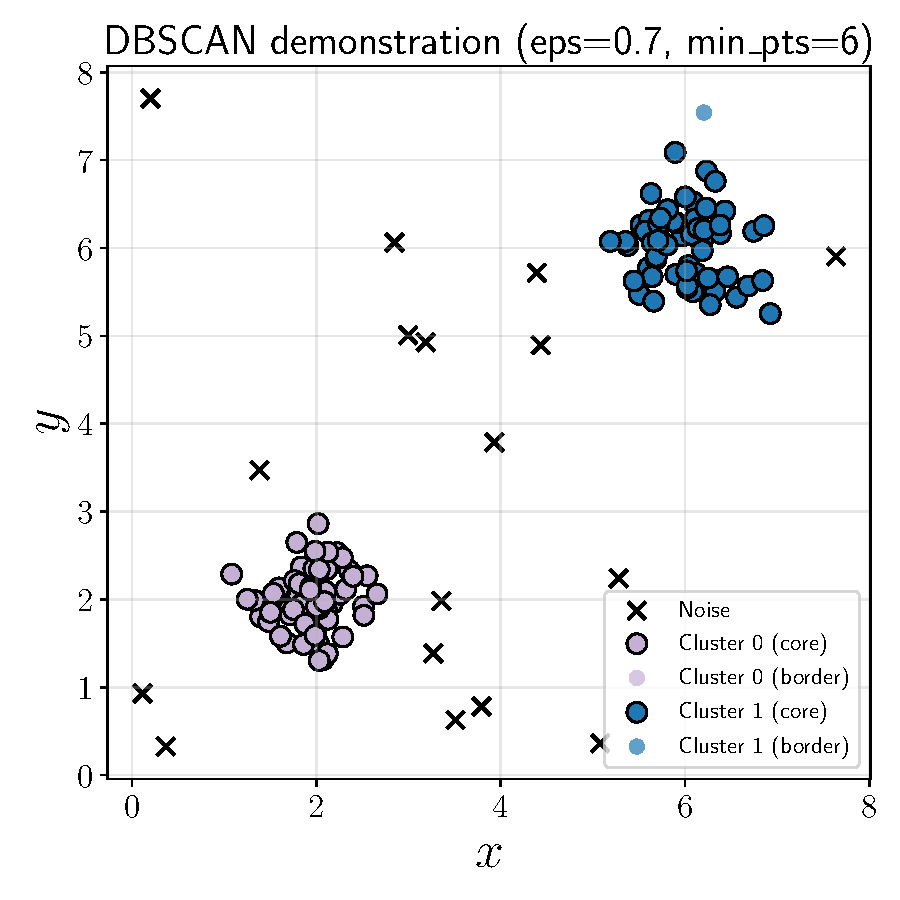
\includegraphics[width=0.4\textwidth]{DBSCAN_illustration.pdf}
  \caption{Schematic illustration on the DBSCAN clustering analysis of 2D data, in which points aggregated in high-density regions are classified into the `core' points, points that are close to the `core' points are classified into the `boarder' points, and the remaining points are classified as `noise'.}
  \label{fig:DBSCAN_clustering}
\end{figure}

Instead of assigning points into clusters based on the distances to the cluster centroids, the DBSCAN clustering algorithm (\cref{fig:DBSCAN_clustering}) adopts a density-based approach to classify points into clusters. The algorithm requirws the pre-definitions of parameters of $\varepsilon$, which defines the radius within which to find the neighbouring points for a given centre, and \texttt{minpts}, which defines the minimum number of points required to form a dense region (or a cluster). Starting from a given data point $\bm{x}_i$, if there are at least \texttt{minpts} data points within the radius of $\varepsilon$ from $\bm{x}_i$, then $\bm{x}_i$ is classified as a `core' point, and all the data points within the radius of $\varepsilon$ from $\bm{x}_i$ are classified as `boarder' points. If there are less than \texttt{minpts} data points within the radius of $\varepsilon$ from $\bm{x}_i$, then $\bm{x}_i$ is classified as a `noise' point. The process is repeated for all the data points until all the points are classified into either `core', `boarder', or `noise' points. The clusters can be formed by connecting the `core' points together, and including the `boarder' points that are close to the `core' points, while excluding the `noise' points. 

In its hierachical variant, the HDBSCAN\cite{campello2015hierarchical} algorithm, it remove the specific requirement for predefining the $\varepsilon$ parameter. Instead, it perform clustering across \textit{many different levels} of $\varepsilon$ and build a hierarchical tree of clusters based on the denisties. From this hierarchical tree, the most stable clusters can be identified based on the stability of the clusters across different levels of $\varepsilon$, which can be quantified by the persistence of the clusters across different levels of $\varepsilon$. 

